\lab{Numerical Methods for Initial Value Problems; Harmonic Oscillators}{Numerical Methods for Initial Value Problems; Harmonic Oscillators}
\label{lab:ivp}

\objective{Implement several basic numerical methods for initial value problems (IVPs), and use them to study harmonic oscillators.}

\section*{Methods for Initial Value Problems}
Consider the initial value problem
\begin{align}
	\begin{split}
y' &= f(x,y),\quad a \leq x \leq b, \\
y(a) &= y_0, 
	\end{split}\label{ivp:generic}
\end{align}
where $f$ is a continuous function. 
A solution of \eqref{ivp:generic} is a continuously differentiable function $y(x)$ that satisfies the equation $y' = f(x,y)$ on the interval $[a,b]$ and for which $y(a) = y_0$. 
In this lab we will focus on numerical methods for approximating $y(x)$, and sidestep the important mathematical problem of verifying that \eqref{ivp:generic} has a unique solution.

For many IVPs it is impossible to find a closed-form, analytic expression for the solution.
When there is a closed-form expression for the solution, it may not be very useful.
In both cases, numerical methods must be relied on to understand the solutions of \eqref{ivp:generic}. 

As an example, consider the initial value problem
\begin{align}
	\begin{split}
y'(x) &= \sin y(x), \\
y(0) &= y_0.
	\end{split}\label{ivp:example}
\end{align}
The solution $y(x)$ is defined implicitly by
\[x = \ln \left|\frac{\cos y_0 + \cot y_0}{\csc y + \cot y} \right|.\]
This analytic expression does not provide much intuition, so we turn to a combination of qualitative and numerical methods. 
Since $\sin (n \pi) = 0$, this differential equation has constant solutions $y_n(x) = n \pi,$ $n \in \mathbb{N}$. 
We can also use an IVP solver to numerically approximate solutions for several other initial values. 
After plotting these solutions (see Figure \ref{ivp:int_curves}), it becomes obvious how solutions of \eqref{ivp:example} behave in general.

\begin{figure}
\centering
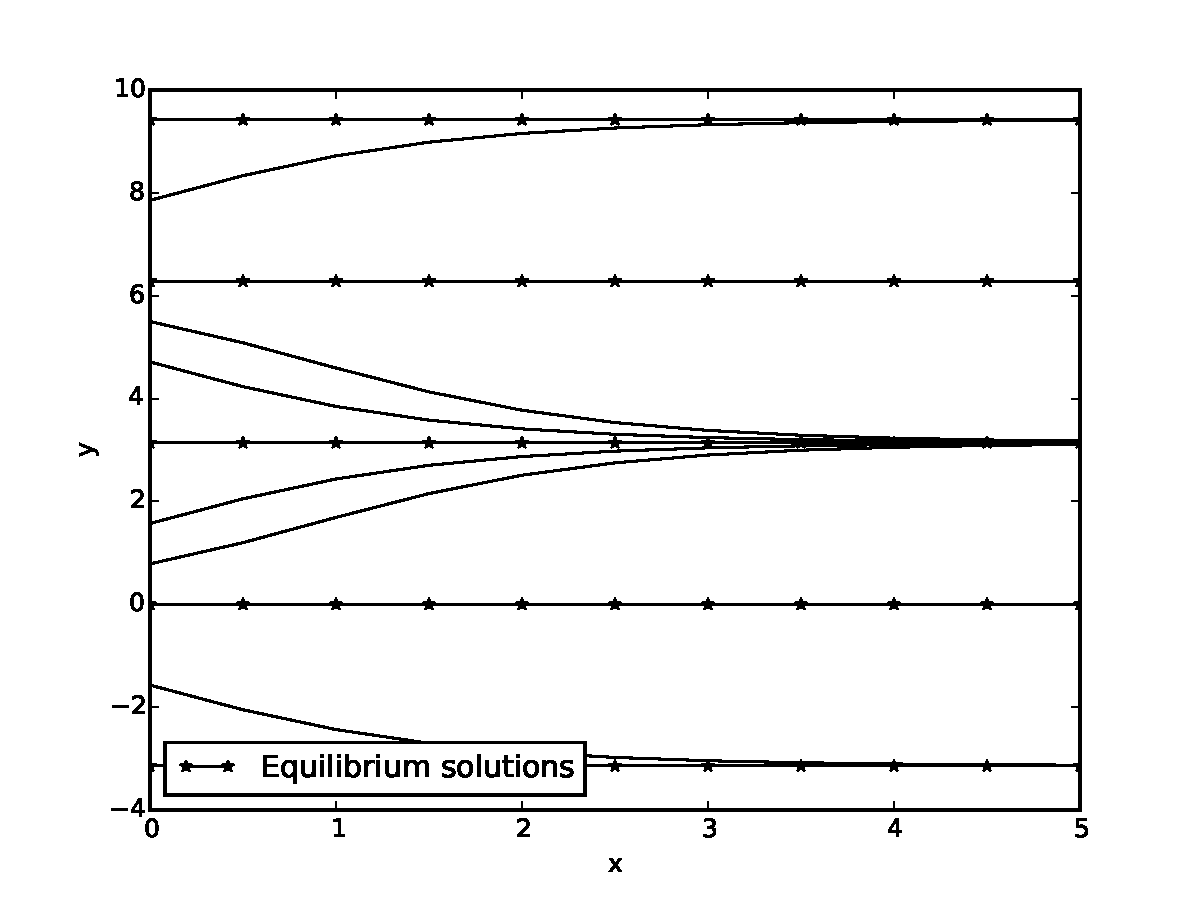
\includegraphics[width=\textwidth]{example.pdf}
\caption{Several solutions of \eqref{ivp:example}, using Numpy's IVP solver \li{dopri5}. }
\label{ivp:int_curves}
\end{figure}


\section*{Numerical Methods}
Numerical methods for solving initial value problems require us to approximate the solution on a set of grid points $a = x_0< x_1<\hdots< x_n = b$ in our interval.  
For simplicity we will assume that each of the $n$ subintervals $[x_{i-1},x_i]$ has equal length $h = (b-a)/n$. $h$ is called the \textit{step size}. 
We then look for values $y_0, y_1, \hdots, y_n$ that approximate the solution at the grid points.
For each $i$, Taylor's theorem says that
\begin{align*}
y(x_{i+1}) &= y(x_{i}) + h y'(x_i) + \frac{h^2}{2} y''(\xi_i)\text{ for some }\xi_i \in [x_i,x_{i+1}].
\end{align*}
The quantity $\frac{h^2}{2} y''(\xi_i)$ is negligible for small $h$, and thus
\begin{align*}
y(x_{i+1}) &\approx y(x_{i}) + h y'(x_i)  ,\\
&\approx y(x_{i}) + h f(x_i,y(x_i)).
\end{align*}
This approximation leads to a method called Euler's method: Letting $y_0 = y(a)$, $y_{i+1}$ is given by $y_{i+1} = y_i +hf(x_i,y_i)$ for $i = 0, 1, \hdots, n-1$.
Euler's method is a first order method, with error $\mathcal{O}(h^1)$.
% \begin{enumerate}
% \item Let $y_0 = y(a)$.
% \item For $i = 0, 1, \hdots, n-1$, let $y_{i+1} = y_i +hf(x_i,y_i)$.
% \end{enumerate}

A similar application of Taylor's theorem shows that
\begin{align*}
y(x_{i}) &= y(x_{i+1}) - h y'(x_{i+1}) + \frac{h^2}{2} y''(\xi_i) \text{ for some } \xi_i \in [x_i,x_{i+1}]; \\
\end{align*}
thus for small $h$
\begin{align*}
y(x_{i+1}) &\approx  y(x_{i}) + h f(x_{i+1},y(x_{i+1})).
\end{align*}
This approximation leads to another first order method called the backwards Euler method: Letting $y_0 = y(a)$, for $i = 0, \hdots, n-1$ we  solve  $y_{i} = y_{i+1}-hf(x_{i+1},y_{i+1})$ for $y_{i+1}$.

Note that for both the Euler and backwards Euler methods, only $y_i, f,$ and other points in the interval $[x_i, x_{i+1}]$ are needed to find $y_{i+1}$. 
Because of this, they are called \textit{one-step methods}.

Euler's method is an \textit{explicit method}. 
The backwards Euler method is an \textit{implicit method} since an equation must be solved at each step to find $y_{i+1}$. 
Explicit and implicit methods each have advantages and disadvantages. 
While implicit methods require an equation to be solved at each time step, they often have better stability properties than explicit methods.

\begin{figure}[ht]
\centering
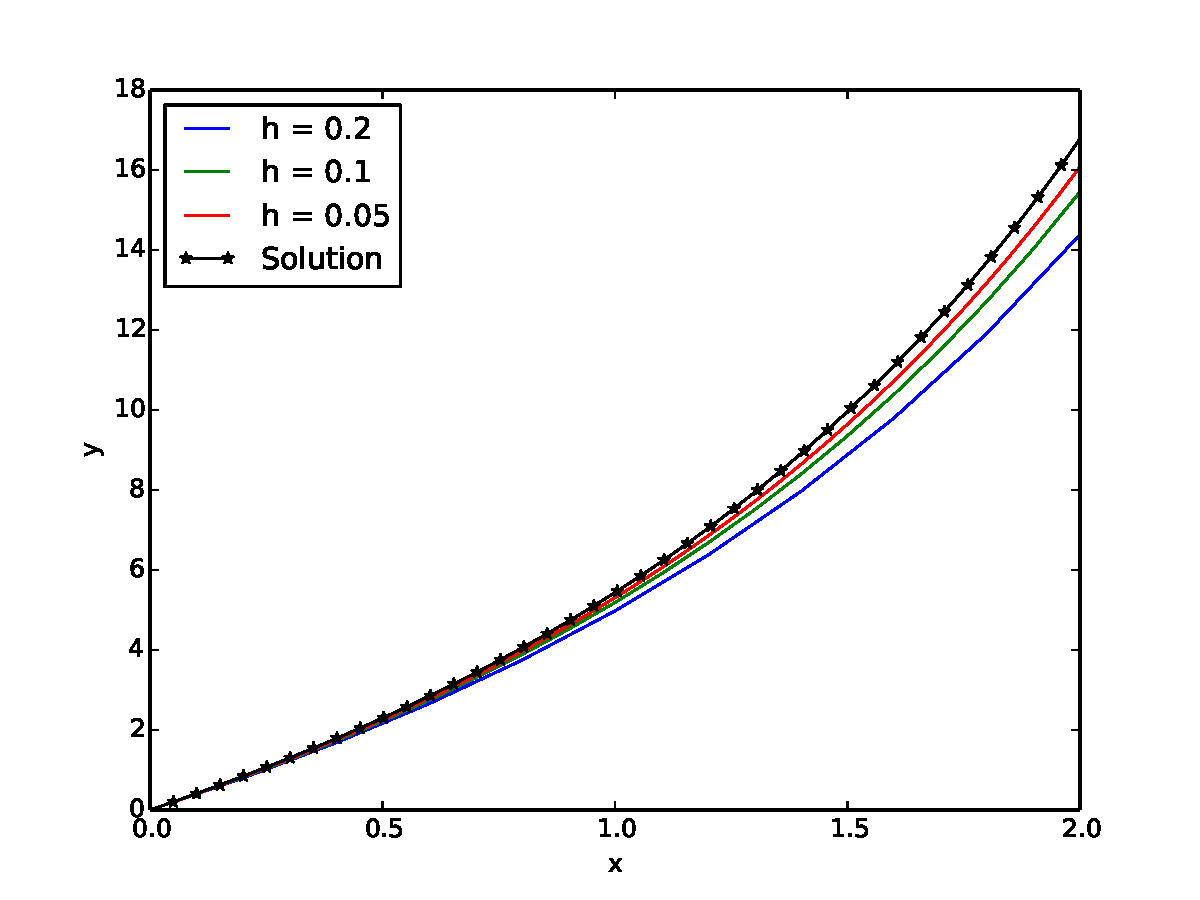
\includegraphics[width=\textwidth]{prob1.pdf}
\caption{The solution of \eqref{ivp:prob1}, alongside several approximations using Euler's method.}
\label{ivp:euler}
\end{figure}


\begin{problem} The solution of
\begin{align}
	\begin{split}
		y' &= y - 2x + 4,\quad 0 \leq x \leq 2, \\
		y(0) &= 0,
	\end{split}\label{ivp:prob1}
\end{align}
is given by $y(x) = -2+2x + 2e^x.$
Use Euler's method to numerically approximate the solution with step sizes $h = 0.4, 0.2$, and $0.1.$ 
Check that your results match Figure \ref{ivp:euler}.
\end{problem}

So how do we come up with numerical methods with higher order accuracy? 
Using Taylor's theorem (as we did for Euler's method) to create higher-order one-step methods would lead to numerically approximating derivatives of $f(t,y)$ - not very desirable.

Let us look for a second order method of the form $y_{i+1} = y_i + a f(x_i+b, y_i+c)$. 
By expanding $a f(x+b, y+c)$ with Taylor's theorem and matching constants in the equation
\begin{align*}
f(x,y) + \frac{h}{2}f'(x,y) &= f(x,y) + \frac{h}{2}\frac{\partial f}{\partial x}(x,y) + \frac{h}{2}\frac{\partial f}{\partial y}(x,y) \cdot f(x,y),
\end{align*}
we find that $a = h, b = h/2,$ and $c = h/2$. 
This method is called the Midpoint method. 
IVP solvers with this general form are called \textit{Runge-Kutta methods}. 
% Another second order Runge-Kutta method is the modified Euler method:
% $y_{i+1} = y_i + \frac{h}{2}[ f(x_i, y_i) + f(x_{i+1}, y_i+ hf(x_i, y_i))]$

There are many Runge-Kutta methods with varying orders of accuracy. 
Methods of order four or higher are most commonly used. A fourth order Runge-Kutta method iterates as follows: 
\begin{align*}
	\begin{split}
K_1 &= f(x_i,y_i), \\
K_2 &= f(x_i + \frac{h}{2}, y_i + \frac{h}{2} K_1),\\
K_3 &= f(x_i + \frac{h}{2} , y_i + \frac{h}{2} K_2),\\
K_4 &= f(x_{i+1} , y_i + h K_3),\\
y_{i+1} &= y_i + \frac{h}{6}(K_1 + 2K_2 + 2K_3 + K_4).
	\end{split}
\end{align*}

Notice that these methods are doing a type of quadrature where we are sampling the function at different points and then performing computation using the samples and some inherent weights. 
For example, consider a differential equation 
\[ y' = f(t).\]
Since the function $f$ has no $y$ dependence, this is a simple integration problem, and these IVP methods become well known quadrature methods. In this case, Euler's method corresponds to the left hand sum, and backward Euler's method corresponds to the right hand sum. 
The modified Euler and midpoint methods are second order IVP methods that correspond to the trapezoidal and midpoint rules for integration, respectively. RK4 corresponds to Simpson's rule for integration.


\begin{comment}
\begin{problem}
Suppose a differential equation is given by
\[ y' = f(t).\]
Since the function $f$ has no $y$ dependence, this a simple integration problem. 
Which integration approximation methods correspond to Euler's method, backward Euler's method, modified Euler's method, the Midpoint method, and the fourth order Runge-Kutta method (RK4)?
\end{problem}
\end{comment}



\section*{Advantages of Higher-Order Methods} 

Higher-order methods are usually much more efficient. One way to measure this efficiency is to determine how many times the right hand side of the initial value problem must be evaluated to provide a desired accuracy.  As an example, consider the initial value problem 
\begin{align}
	\begin{split}
		y' &= y \cos(x), x \in [0,8],\\
		y(0) &= 1. 
	\end{split}
	\label{ivp:efficiency_problem}
\end{align}
Figure \ref{ivp:efficiency_figure} illustrates the comparative efficiency of the Euler, Midpoint, and RK4 methods.  The figure also demonstrates another point: since the lower order methods require more floating point operations, floating point error limits the highest possible accuracy that can be achieved with lower order methods. 

\begin{figure}[ht]
\centering
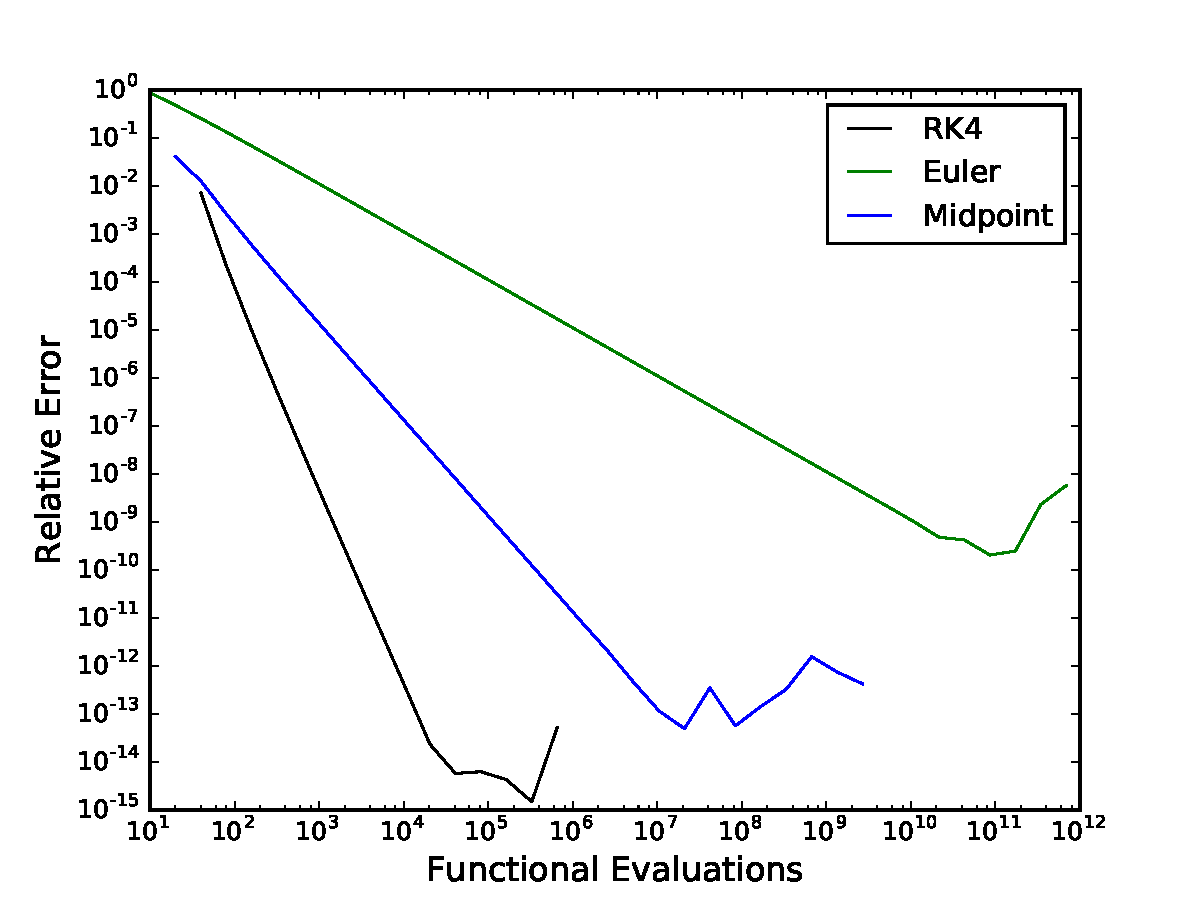
\includegraphics[width=\textwidth]{Efficiency.pdf}
\caption{Here we graph the relative error in computing the solution of \eqref{ivp:efficiency_problem} at $x = 8$, versus the number of times the right side of \eqref{ivp:efficiency_problem} must be evaluated.  }
\label{ivp:efficiency_figure}
\end{figure}




Let $t^*$ be an approximation of some value $t$. The relative error of the approximation is 
\[ \frac{|t^*-t|}{|t|}.
\]
Note that the relative error is simply the absolute error $|t^*-t|$ normalized by the size of $t$.  A method with order $p$ has error of the form 
\[E(h) = C h^p. \]
This means that the graph of $\log (E)$ versus $\log(h)$ has slope $p$.  
The relative error of a numerical method can be approximated and graphed to verify that $p$th order convergence is occurring. For example, consider the IVP
 \begin{align}
 	\begin{split}
 y' &= y - 2x + 4,\quad 0 \leq x \leq 2, \\
 y(0) &= 0.
 	\end{split} \label{ivp:prob2}
 \end{align}
The following code solves the initial value problem on several grids using the Euler method, approximates the relative error in computing $y(2)$ and creates a plot (see Figure \ref{ivp:relative_error}).

\begin{lstlisting}
import matplotlib.pyplot as plt

a, b, ya = 0., 2., 0.

def ode_f(x,y):
	return np.array([y -2*x + 4.])
	
best_grid = 320					#  number of subintervals in most refined grid
# Requires an implementation of the euler method
best_val = euler(ode_f,ya,a,b,best_grid)[-1]  

smaller_grids = [10,20,40,80]  # number of subintervals in smaller grids
h = [2./N for N in smaller_grids]
Euler_sol = [euler(ode_f,ya,a,b,N)[-1] for N in smaller_grids]
Euler_error = [abs(( val - best_val)/best_val ) for val in Euler_sol]
	
plt.loglog(h, Euler_error, '-b', label="Euler method"	  , linewidth=2.)
plt.show()

\end{lstlisting}


\begin{problem} Consider the IVP \eqref{ivp:prob2}.
Use the Midpoint method and the fourth order Runge-Kutta method (RK4) to approximate the value of the solution at $x = 2$, with a step size of $h = 0.2,$ $ 0.1,$ $0.05 $, $0.025,$ and $0.0125.$ 
Create a log-log plot of the relative error of each approximation using the \li{loglog} function in \li{matplotlib} (see Figure \ref{ivp:relative_error}).
\end{problem}

\begin{figure}[ht]
\centering
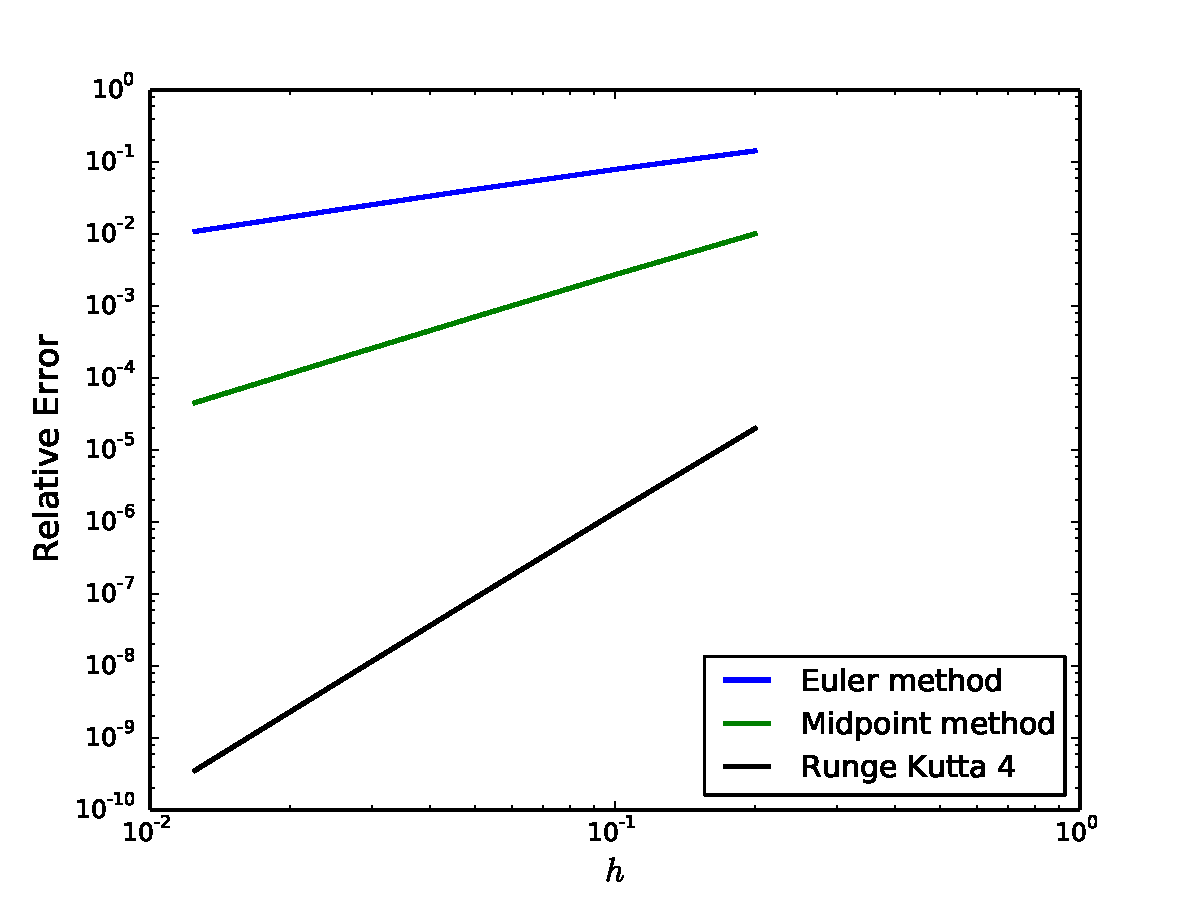
\includegraphics[width=\textwidth]{relative_error.pdf}
\caption{The solution of $y' -y= -2x+4,$ $y(0) = 0$, is $y(x) = -2+2x + 2e^x.$ This loglog plot shows the relative error in numerically approximating $y(2)$, using step sizes $h = 0.2,$ $0.1,$ $0.05,$ $0.025,$ and $0.0125$. The slope of each line demonstrates the first, second, and fourth order convergence of the Euler, Midpoint, and RK4 methods, respectively.}
\label{ivp:relative_error}
\end{figure}


\section*{Harmonic Oscillators and Resonance} 
Harmonic oscillators show up often in classical mechanics.
A few examples include the pendulum (with small
 displacement), spring-mass systems, and the flow of electric current through various types of circuits.
A harmonic oscillator can be described by an initial value problem of the form
\begin{align*}
	&{}my'' + \gamma y' + ky = f(t) ,\\
	&{}y(0) = y_0,\quad
	y'(0) = y'_0.
\end{align*}
We will describe the construction of this mathematical model in the context of a spring-mass system.

Suppose an object with mass $m$ is placed at the end of a horizontal spring.
The natural position of the object is called the \textit{equilibrium position} for the system.
If the object is displaced from its equilibrium position and given an initial velocity,
it will act like a harmonic oscillator.
The principal property of a harmonic oscillator $y(t)$ is that once $y$ leaves its equilibrium value $y = 0$, it experiences a restoring force $F_r = -ky.$
This force pushes $y$ back towards its equilibrium.
Hooke's law says that this holds true for a
spring-mass system if the displacement $y$ is small.

Often there is an additional damping force $F_d$, often due to some type of friction. 
This force is usually proportional to the $y'$ (the \emph{velocity}), is always in the opposite direction of $y'$, and represents energy leaving the system. (You can think of it as drag.)
Thus we have $F_d = -\gamma y', $ where $ \gamma \geq 0$ is constant.
We may also need to consider an additional external force $f(t)$, or a driving force, that is interacting with our spring-mass system.

By using Newton's law we obtain
\begin{align*}
ma &= F = F_r + F_d + f(t),\\
my'' &= -ky -\gamma y' + f(t).
\end{align*}

\section*{Simple harmonic oscillators}
A simple harmonic oscillator is a harmonic oscillator that is not damped ($\gamma =0$), and is free ($f = 0$) rather than forced ($f \not = 0$). 
A simple harmonic oscillator can described by the IVP
\begin{align*}
&{}my'' + ky = 0,\\
&{}y(0) = y_0,\quad
y'(0) = y_0'.
\end{align*}
The solution of this IVP is $y = c_1\cos (\omega_0 t) + c_2 \sin (\omega_0 t)$ where $\omega_0 = \sqrt{k/m}$ is the natural frequency of the oscillator and $c_1$ and $c_2$ are determined by applying the initial conditions. This in turn can be written in the form
\[y = A\sin (\omega_0 t + \delta) .\]

To solve this IVP using the fourth order Runge Kutta method (RK4), we need to write this system in the form
\[z'(t) = f(t,z(t)) \]
We can do this by letting $z_1 = y, z_2 = y'$. Then we have \[     z'=
 \left[\begin{array}{c}z_1 \\z_2\end{array}\right]'  =  \left[\begin{array}{c}z_2 \\\frac{-k}{m}z_1\end{array}\right]= f(z).\]


\begin{problem} Use the RK4 method to solve for the simple harmonic oscillator satisfying 
\begin{align}
	\begin{split}
&{}my'' + ky = 0,\quad 0 \leq t \leq 20, \\
&{}y(0) = 2, \quad
y'(0) = -1,
	\end{split}
	\label{ivp:simple_oscillator}
\end{align}
for $m = 1$ and $k =1$. Note that in your implementation of RK4, the constants $K_1, K_2, K_3,$ and $K_4$ become vectors with $n$ entries, where $n$ is the number of equations in the first-order system.

Plot your numerical approximation of $y(t)$.  
Compare this with its numerical approximation when $m = 3$ and $k =1$. Consider: Why does the difference in solutions make sense physically?
\end{problem}


\begin{figure}[ht]
\centering
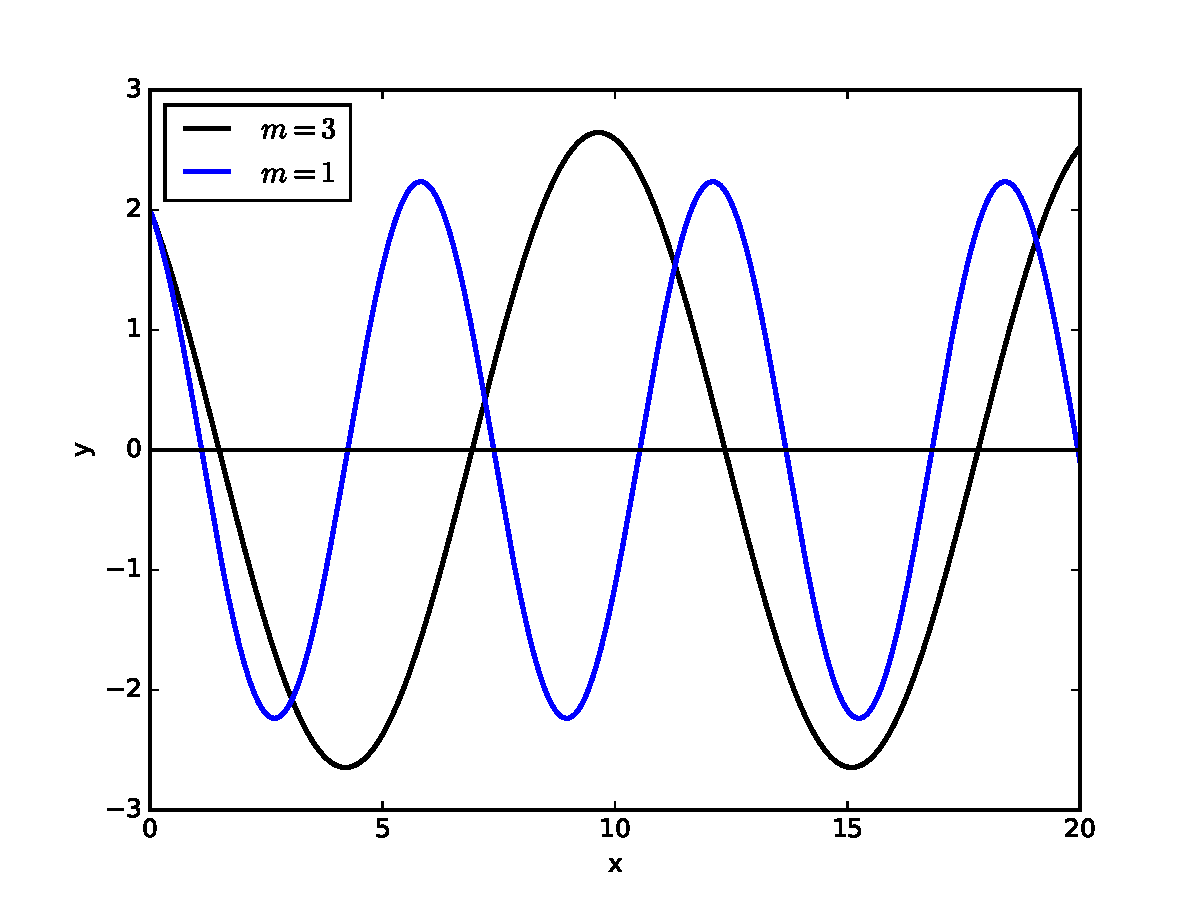
\includegraphics[width=\textwidth]{simple_oscillator.pdf}
\caption{Solutions of \eqref{ivp:simple_oscillator} for several values of $m$.}
\label{ivp:simple_oscillator_figure}
\end{figure}


\section*{Damped free harmonic oscillators} 
We now consider damped free harmonic oscillators. 
These systems are described by the differential equation
\[my''(t) +\gamma y'(t) + ky(t) = 0.\]
For fixed values of $m$ and $k$, it is interesting to study the effect of the damping coefficient $\gamma$.

The roots of the characteristic equation are \[r_1,r_2 = \frac{-\gamma \pm \sqrt{\gamma^2 -4km}}{2m} .\]
Note that the real parts of $r_1$ and $r_2$ are always negative, and so any solution $y(t)$ will decay over time due to a dissipation of the system energy. 
There are several cases to consider for the general solution of this equation:
\begin{enumerate}
\item If $\gamma^2 > 4km$, then the general solution is $y(t) = c_1 e^{r_1t} + c_2e^{r_2t}$. Here the system is said to be $\textit{overdamped}$. 
Notice from the general solution that there is no oscillation in this case.
\item If $\gamma^2 = 4km$, then the general solution is $y(t) = c_1 e^{\gamma t/2m} + c_2 te^{\gamma t/2m}$. Here the system is said to be $\textit{critically damped}$.
\item If $\gamma^2 < 4km$, then the general solution is
\begin{align*}
y(t) &= e^{-\gamma t/2m} \left[c_1\cos(\mu t) + c_2 \sin (\mu t)\right],\\
&= R e^{-\gamma t/2m}  \sin (\mu t + \delta),
\end{align*}
where $R$ and $\delta$ are fixed, and $\mu = \sqrt{4km-\gamma^2}/2m.$ This system does oscillate.
\end{enumerate}

\begin{problem}
Use the RK4 method to solve for the damped free harmonic oscillator satisfying 
\begin{align*}
&{}y'' +\gamma y'+ y = 0, \quad 0 \leq t \leq 20,\\
&{}y(0) = 1, \quad
y'(0) = -1.
\end{align*}
For $\gamma = 1/2,$ and $\gamma = 1$, simultaneously plot your numerical approximations of $y$.  
Find $y(20)$ accurate to four significant digits, by checking that the relative error is less than $5\times 10^{-5}$.  
How many subintervals do you need?
\end{problem}

\section*{Forced harmonic oscillators without damping}
Let's look at the systems described by the differential equation
\begin{align}
my''(t)  + ky(t) &= F(t). \label{Forced_harm_osc}
\end{align}
In many instances the external force $F(t)$ is periodic, so let us assume that $F(t) = F_0 \cos(\omega t)$. 
If $\omega_0 = \sqrt{k/m} \not = \omega,$ then the  general solution of \ref{Forced_harm_osc} is given by
\[y(t) = c_1 \cos (\omega_0 t) + c_2\sin (\omega_0 t) + \frac{F_0}{m(\omega_0^2 - \omega^2)} \cos (\omega t).\]
If $\omega_0 = \omega$, then the general solution is
\[y(t) = c_1 \cos (\omega_0 t) + c_2\sin (\omega_0 t) + \frac{F_0}{2m\omega_0} t \sin (\omega_0 t).\]

In the case that $\omega_0 = \omega$, the solution contains a term that grows arbitrarily large as $t \to \infty$.
If we included damping then the solution would be bounded, but would still be large for small $\gamma$ and $\omega$ close to $\omega_0$.

Consider a physical spring-mass system.
Equation \ref{Forced_harm_osc} holds only for small oscillations (this is where Hooke's law is applicable).
For larger oscillations, this equation will not hold.
However, the fact that the equation predicts large oscillations suggests the spring-mass system could fall apart as a result of the external force. 
Mechanical resonance has been known to cause failure of bridges, buildings, and airplanes.

\begin{problem}
Use the RK4 method to solve for the damped and forced harmonic oscillator satisfying 
\begin{align}
	\begin{split}
&{}2y'' + \gamma y' + 2y = 2 \cos (\omega t), \quad 0 \leq t \leq 40,\\
&{}y(0) = 2, \quad
y'(0) = -1. 
	\end{split}
	\label{ivp:damped_forced_oscillator}
\end{align}
For the following values of $\gamma$ and $\omega,$ plot your numerical approximations of $y$ and find $y(40)$ accurate to four significant digits: $(\gamma, \omega) = (0.5, 1.5),$ $(0.1, 1.1),$ and $(0, 1).$
\end{problem}


\begin{figure}[ht]
\centering
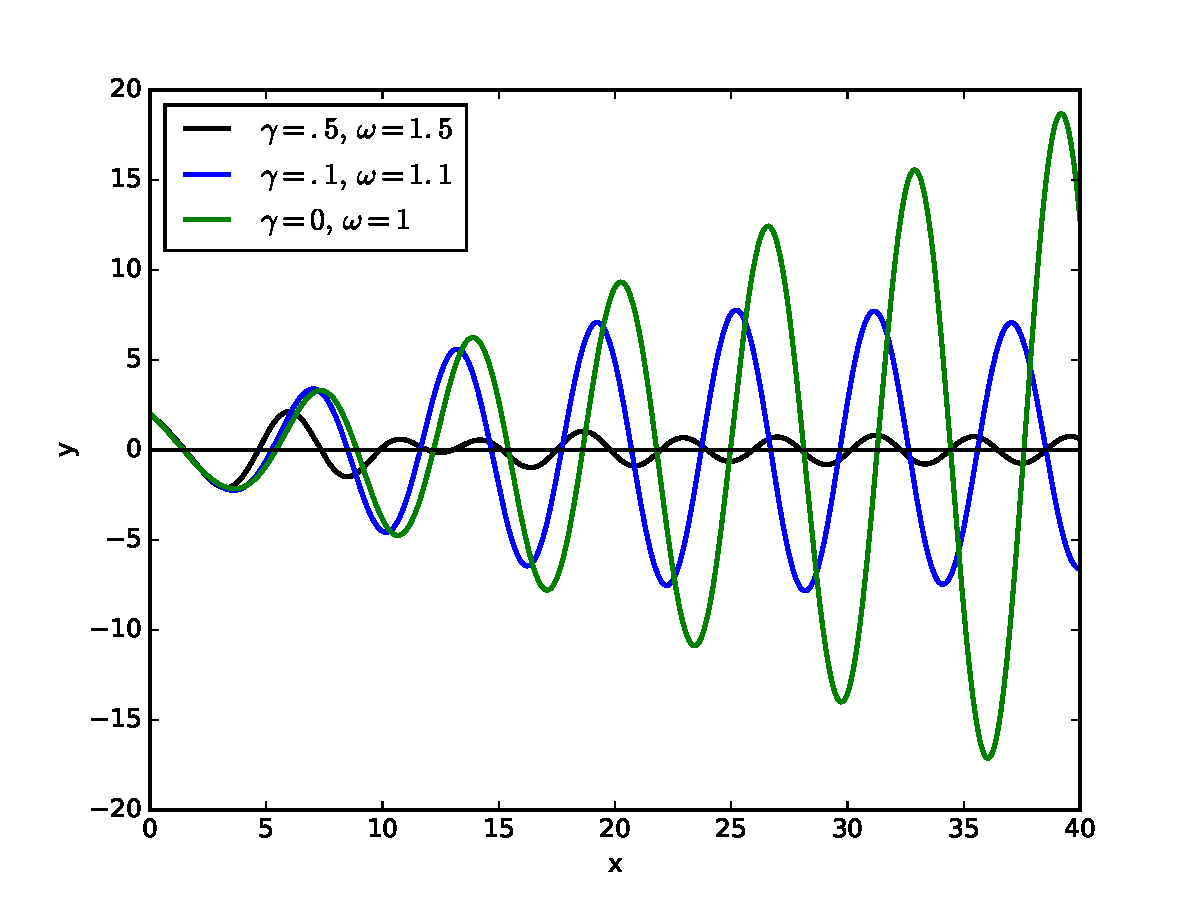
\includegraphics[width=\textwidth]{damped_forced_oscillator.pdf}
\caption{Solutions of \eqref{ivp:damped_forced_oscillator} for several values of $\omega$ and $\gamma$.}
\label{ivp:damped_forced_oscillator_figure}
\end{figure}
